

\tikzset{every picture/.style={line width=0.75pt}} %set default line width to 0.75pt        

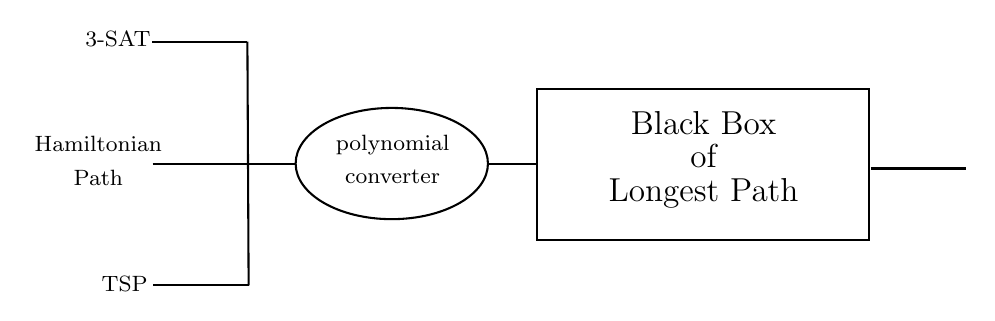
\begin{tikzpicture}[x=0.75pt,y=0.75pt,yscale=-0.8,xscale=0.85]
%uncomment if require: \path (0,190); %set diagram left start at 0, and has height of 190

%Shape: Rectangle [id:dp5858986987668833] 
\draw   (346,48.2) -- (534.3,48.2) -- (534.3,139.2) -- (346,139.2) -- cycle ;
%Straight Lines [id:da46696467690404164] 
\draw    (182.3,93.2) -- (209.3,93.2) ;
%Straight Lines [id:da7226282801894859] 
\draw    (181.95,19.8) -- (182.65,166.6) ;
%Straight Lines [id:da24655226707604183] 
\draw    (127.95,19.8) -- (181.95,19.8) ;
%Straight Lines [id:da31820252404488514] 
\draw    (128.3,93.2) -- (182.3,93.2) ;
%Straight Lines [id:da24681491849861903] 
\draw    (128.65,166.6) -- (182.65,166.6) ;
%Straight Lines [id:da9371672251683474] 
\draw    (535.3,96.2) -- (589.3,96.2) ;
%Shape: Ellipse [id:dp28899224478328267] 
\draw   (209.3,93.2) .. controls (209.3,74.7) and (233.7,59.7) .. (263.8,59.7) .. controls (293.9,59.7) and (318.3,74.7) .. (318.3,93.2) .. controls (318.3,111.7) and (293.9,126.7) .. (263.8,126.7) .. controls (233.7,126.7) and (209.3,111.7) .. (209.3,93.2) -- cycle ;

%Straight Lines [id:da8470962010892356] 
\draw    (318.3,93.2) -- (345.3,93.2) ;

% Text Node
\draw (58,75) node [anchor=north west][inner sep=0.75pt]   [align=left] {\begin{minipage}[lt]{48.07600000000001pt}\setlength\topsep{0pt}
\begin{center}
{\footnotesize Hamiltonian }\\{\footnotesize Path}
\end{center}

\end{minipage}};
% Text Node
\draw (96,159) node [anchor=north west][inner sep=0.75pt]   [align=left] {\begin{minipage}[lt]{18.598000000000003pt}\setlength\topsep{0pt}
\begin{center}
{\footnotesize TSP}
\end{center}

\end{minipage}};
% Text Node
\draw (87,12) node [anchor=north west][inner sep=0.75pt]   [align=left] {\begin{minipage}[lt]{25.245pt}\setlength\topsep{0pt}
\begin{center}
{\footnotesize 3-SAT}
\end{center}

\end{minipage}};
% Text Node
\draw (380,60) node [anchor=north west][inner sep=0.75pt]   [align=left] {\begin{minipage}[lt]{74.85984pt}\setlength\topsep{0pt}
\begin{center}
{\large Black Box }\\{\large of }\\{\large Longest Path}
\end{center}

\end{minipage}};
% Text Node
\draw (228,74) node [anchor=north west][inner sep=0.75pt]   [align=left] {\begin{minipage}[lt]{43.996pt}\setlength\topsep{0pt}
\begin{center}
{\footnotesize polynomial }\\{\footnotesize converter}
\end{center}

\end{minipage}};


\end{tikzpicture}